%% ****** Start of file apstemplate.tex ****** %
%%
%%
%%   This file is part of the APS files in the REVTeX 4 distribution.
%%   Version 4.1r of REVTeX, August 2010
%%
%%
%%   Copyright (c) 2001, 2009, 2010 The American Physical Society.
%%
%%   See the REVTeX 4 README file for restrictions and more information.
%%
%
% This is a template for producing manuscripts for use with REVTEX 4.0
% Copy this file to another name and then work on that file.
% That way, you always have this original template file to use.
%
% Group addresses by affiliation; use superscriptaddress for long
% author lists, or if there are many overlapping affiliations.
% For Phys. Rev. appearance, change preprint to twocolumn.
% Choose pra, prb, prc, prd, pre, prl, prstab, prstper, or rmp for journal
%  Add 'draft' option to mark overfull boxes with black boxes
%  Add 'showpacs' option to make PACS codes appear
%  Add 'showkeys' option to make keywords appear
% \documentclass[aps,prl,preprint,groupedaddress]{revtex4-1}
%\documentclass[aps,prl,preprint,superscriptaddress]{revtex4-1}
%\documentclass[aps,prl,reprint,groupedaddress]{revtex4-1}

\documentclass[%
 reprint,
%superscriptaddress,
%groupedaddress,
%unsortedaddress,
%runinaddress,
%frontmatterverbose,
%preprint,
%showpacs,preprintnumbers,
%nofootinbib,
%nobibnotes,
%bibnotes,
 amsmath,amssymb,
 aps,
%pra,
%prb,
prl
%rmp,
%prstab,
%prstper,
%floatfix,
]{revtex4-1}


\usepackage{epsfig}
\usepackage{natbib}
\usepackage{subfig}
\usepackage[]{graphicx}
\usepackage{rotating}
\usepackage{here}
\usepackage{calc}
\usepackage{multirow}
\usepackage{amsfonts}
\usepackage{amssymb}
\usepackage{color}
\usepackage{nomencl}
\usepackage{textcomp}
\usepackage{eurosym}
\usepackage[ansinew]{inputenc}
\usepackage[bookmarks=true,bookmarksnumbered=true]{hyperref}

\graphicspath{{figures/EPS/}}


% You should use BibTeX and apsrev.bst for references
% Choosing a journal automatically selects the correct APS
% BibTeX style file (bst file), so only uncomment the line
% below if necessary.
%\bibliographystyle{apsrev4-1}

\begin{document}

% Use the \preprint command to place your local institutional report
% number in the upper righthand corner of the title page in preprint mode.
% Multiple \preprint commands are allowed.
% Use the 'preprintnumbers' class option to override journal defaults
% to display numbers if necessary
%\preprint{}

%Title of paper
\title{Stability analysis for free surface flows}

% repeat the \author .. \affiliation  etc. as needed
% \email, \thanks, \homepage, \altaffiliation all apply to the current
% author. Explanatory text should go in the []'s, actual e-mail
% address or url should go in the {}'s for \email and \homepage.
% Please use the appropriate macro foreach each type of information

% \affiliation command applies to all authors since the last
% \affiliation command. The \affiliation command should follow the
% other information
% \affiliation can be followed by \email, \homepage, \thanks as well.
\author{Leo M. Gonz\'alez}
 \email{leo.gonzalez@upm.es}
\affiliation{%
  Naval Architecture Department (ETSIN)\\
  Technical University of Madrid (UPM)\\
  Arco de la Victoria s/n, 28040 Madrid, Spain
}%

\author{Juan M. Gimenez}
\email{jmarcelogimenez@gmail.com}
\affiliation{
Centro de Investigaci\'on de M\'etodos Computacionales (CIMEC) - UNL/CONICET \\
Predio Conicet-Santa Fe Colectora Ruta Nac 168 \\
Paraje El Pozo, Santa Fe, Argentina\\
}%
\affiliation{
 Facultad de Ingenier\'ia y Ciencias H\'idricas\\
 Universidad Nacional del Litoral, Santa Fe, Argentina
}

\date{\today}% It is always \today, today,
             %  but any date may be explicitly specified

\begin{abstract}
This Letter describes how the results of a global stability analysis of a classical circular cylinder are affected when the cylinder submerged and a two phase flow is present. The two phase flow has been transformed into a single phase fluid with variable density and viscosity using a volume of fluid (VOF) characterization. The Navier-Stokes equations which depend on both the Reynolds and Froude numbers, have been fixed to create a particular scenario for the stability analysis. Consequently, the baseflow obtained by the Navier-Stokes equations have been analyzed and the Hopf bifurcation has been obtained for a particular Froude number. The critical Reynolds number and the frequency of the most unstable mode have been compared to the classical solution without free surface.
\end{abstract}

% insert suggested PACS numbers in braces on next line
\pacs{}
% insert suggested keywords - APS authors don't need to do this
%\keywords{}

%\maketitle must follow title, authors, abstract, \pacs, and \keywords
\maketitle

%=====================================================================================
\section{Introduction}
\label{S:Intro}
%=====================================================================================

The interaction between the viscous wake of a submerged object and the free surface position is a problem that deserves a serious study. Several reasons sustain this importance, \cite{Dimas89} justifies the study due to its potential relevance for the remote sensing of the ocean surface from satellites while \cite{Reichl05,Bouscasse14} also underline its application to the design of offshore structures and vessels.
It is well known that in the absence of free surface the von Karman vortex street generated by flow past an infinitely long circular cylinder produces a two dimensional time periodic flow for Reynolds numbers between approximately 47 and 189 \cite{JacksonJFM87,ProvansalJFM87,WilliamsonPoF88,miller1994control}. The Reynolds number is quantified as $Re= U_\infty D/\nu$ , where $U_\infty$ the fluid velocity far from the cylinder, $D$ is the cylinder diameter, and $\nu$ is the kinematic viscosity. This work is focused on analyzing the changes produced in this flow when the cylinder is submerged and a free surface separating two different fluids in the presence of gravity. Different steady baseflows have been studied and a linear global stability analysis has been performed in order to quantify the differences when free surface and gravity are added to the problem. Previous authors performed stability analysis of idealized problems such as simple vortex structures \cite{ohring1991interaction,fontane2008stability} and analytic shear flows \cite{Dimas89}. To the authors knowledge it is the first time that a global stability analysis is performed on a Navier-Stokes computed solution in the presence of high discontinuities in density caused by the free surface. In order to gain insight about the basic physics of the interaction, steady flows where the velocity, the pressure and the free surface finally reach a stationary state are analyzed. The problem depends on two non-dimensional numbers, such as the Reynolds and the Froude numbers. The particular case when only one fluid is used has a very well studied solution and the steady separation bubble breaks its stability when the only non-dimensional parameter that appears in this case increases its value over $Re_c=47$. For Reynolds values above this critical number perturbations amplify and the stability of the separation bubble breaks. Taking the critical Reynolds number, $Re_c$ as a reference value without free surface, in our study the Reynolds number has been increased from subcritical to supercritical values  while the Froude number has been kept constant along the study. Two causes could cause the first instability of these flows: typical vortex shedding instability or a free surface instability similar to the Rayleigh case. In our study the range of the main parameters Reynolds and Froude has been selected such that the vortex shedding is the main cause of instability while the free surface only alters the fluid domain setup.
Similarly with the work presented by \cite{Dimas89} here the propose is to analyze the stability of the wake of a floating two-dimensional object. However two main differences can be found between both methodologies, first, in our case no time averaged flow or double body hypothesis has been used for the baseflow, instead, the perturbed base flow has been computed solving the Navier-Stokes equations for the two fluids that are involved in the computation and the Rayleigh equations cannot model the stability analysis. Second, no boundary conditions have been used for the free surface, and a VOF function \cite{hirt1981volume} has been used to simulate the density and viscosity changes. As a continuation of the work perform ed by Dimas, the question of how affects the presence of the free surface -here introduced by a VOF function- the stability of the wake region behind the floating object. Third, a global analysis in the XY plane has been performed consequently not assuming any harmonic dependance of the perturbation in the flow direction.

Dimas-the cylinder is assumed to be half submerged, the experimental velocity profiles of the unbounded flow around a cylinder at Reynolds 140000 were fitted by an anatlytic expression and used for the stability calculations and

%=====================================================================================
\section{Methodology}
\label{S:Methodology}
%=====================================================================================


The governing equations are the incompressible Navier�Stokes equations in laminar regime, which are supplemented with the conventional boundary conditions on solid and/or open boundaries. The computational domain $\Omega$ contains both fluids, the first one denoted by subscript 1 is placed at the top of the domain, and the second one placed at the bottom denoted by the subscript 2. Let us name their corresponding densities and viscosities as $\rho_i$ and $\mu_i$(i=1,2), respectively. The governing equations, written in a Lagrangian framework, are:

\begin{eqnarray}
  \nabla \cdot \mathbf{v} &=& 0 \label{eq:continuity} \\
  \rho\frac{D\mathbf{v}}{Dt} &=& -\nabla p + \mu \nabla^2 \mathbf{v} + \rho \mathbf{g}  \label{eq:momentum}
\end{eqnarray}

Here $\mathbf{v}$, $p$ are the velocity and fluid pressure and $\rho \mathbf{g}$ is the gravity force. Once the equations are written in non-dimensional form using the cylinder diameter $D$, the inflow velocity $U$ and the density and viscosity of the bottom fluid. It is important to remark, that a non dimensional coefficient based on the fluid properties $\alpha$ appears explicitly in the viscous term of the momentum conservation equation. The Reynolds number $Re_D=\frac{UD}{\nu_{b}}$ will be defined by the fluid properties of the bottom fluid. An efficient and accurate methodology, called PFEM-2, has been used to numerically simulate the dynamics of an incompressible flow during the baseflow computation. It is important to remark that both density and viscosity are discontinuous functions that have been transported according to the techniques described in \cite{Gimenez2015186}.

\begin{equation}\label{Viscous coeff}
    \alpha=\frac{(\phi+1)-(\frac{\nu_{t}}{\nu_{b}})(\phi-1)}{2 Re_D}
\end{equation}


It is easy to find derived non dimensional Froude numbers based on the distances $H$, $h$.	



We choose a sufficiently large domain size to minimize the undesirable boundary effects. The inflow and exit boundaries are each located at 18D and 35D towards the fore and aft of the cylinder, respectively. The far field boundary is located at 15D on either side of the central axis. A uniform inflow boundary condition, together with a natural boundary condition for the far field and outflow, are applied for the velocity. The no-slip boundary condition is employed for the non-rotational part of the D cylinder. The Neumann boundary condition is also imposed for the pressure at the exit.

An accurate and efficient simulation of the interface evolution is crucial in the simulation of free-surface flows. During the flow evolution, it is essential that the interface remains sharp. Large jumps of fluid density and viscosity across the interface should be correctly assumed by the numerical algorithm in order to satisfy the momentum balance at the vicinity of the interface. Readers interested in more details of the PFEM-2 method and the enrichment technique used for the free surface definition may see \cite{Gimenez2015186}.

The complete analysis requires two steps: during the first one, the two-dimensional equations of motion are solved for those $Re$ and $Fr$ values that finally reach a final steady state. The stability of those steady basic flows $(\overline{\mathbf{v}}, \overline{p},\overline{\phi})$ will subsequently be investigated. For those cases where the Reynolds number is above the critical value and no steady state is obtained turning to a periodic case, a time averaged solution is analyzed assuming that the analysis is still valid according to \cite{SippLebedev}. During the second step, the basic flow is perturbed by small-amplitude velocity $\widetilde{\mathbf{v}}$ and kinematic pressure $\widetilde{p}$ perturbations, as follows

\begin{eqnarray}
  \mathbf{v} &=& \overline{\mathbf{v}} + \varepsilon \widetilde{\mathbf{v}} \\
  p &=& \overline{p} + \varepsilon \widetilde{p}
\end{eqnarray}

where $\varepsilon\ll 1$. The stability analyses of the equations implies the linearization of the Navier-Stokes equations around a steady base flow. This process has been done following the same methods explained in \cite{Gonzalez07} which implies the resolution of a large generalized eigenvalue problem by an iterative Arnoldi method. However, two important considerations should be remarked when this analysis step is performed:

-The steady baseflow implies a final distribution of both fluids, see figure \ref{free_surface}, that it is quantified by the values of the VOF function. As usual, the free surface is represented by the value 0 of the VOF function. The VOF function determines the kinematic viscosity variation and once the flow has reached a steady situation this distribution is freezed.

-The viscous term depends on the kinematic viscosity distribution, which includes two constant zones representing the air and the water areas, but also an important gradient on the free surface. When the Navier-Stokes equations are solved and perturbed those gradients must be taken into account and new terms depending on the gradient of the kinematic viscosity are not negligible on the free surface proximities.


After a complete mesh converge process, a final mesh where the numerical results are confirmed has been selected. The mesh used for the simulations is a linear triangular mesh that contains 65834 triangles and 132542 nodes, the default mesh size is 0.655D while in the cylinder proximities and the free surface area the mesh size has been refined to 0.0016D. See figure \ref{f:geometryandmesh} to appreciate the mesh configuration.



\begin{figure}[ht]
  \centering
    \subfloat[Case configuration]{
	  \label{case-geo}
	  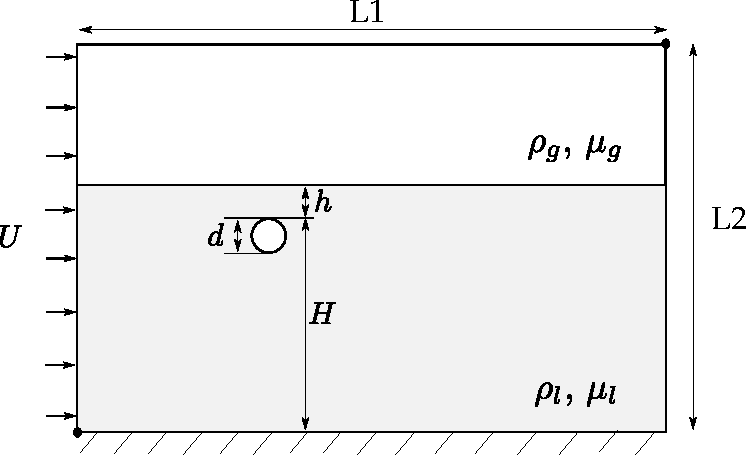
\includegraphics[width=.9\columnwidth]{config.pdf}
    } \\
    %%----segunda subfigura----
    \subfloat[Detailed Mesh]{
	  \label{case-mesh}
	  %\includegraphics[width=.9\columnwidth]{mesh_new.eps}
	  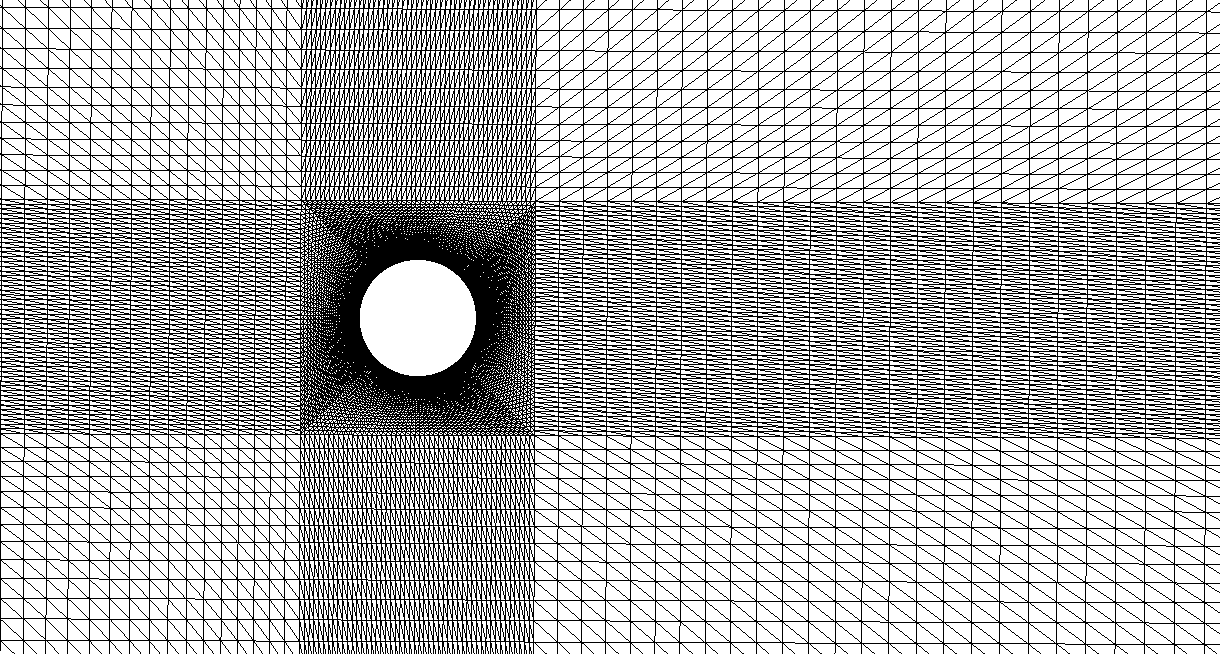
\includegraphics[width=.9\columnwidth]{mesh.png}
    }
    \caption{General and detailed views of the mesh used for the baseflow computation and subsequent analysis, the circular cylinder is submerged a depth $h$.}
   \label{f:geometryandmesh}                %% Etiqueta para la figura entera
\end{figure}

%
% \begin{figure}
% \begin{center}
% \label{f:geometryandmesh}
%   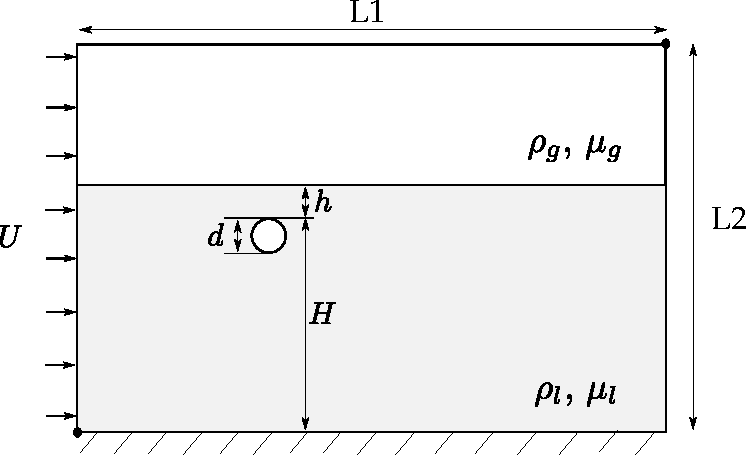
\includegraphics[width=.9\columnwidth]{config.pdf} \\
%
%   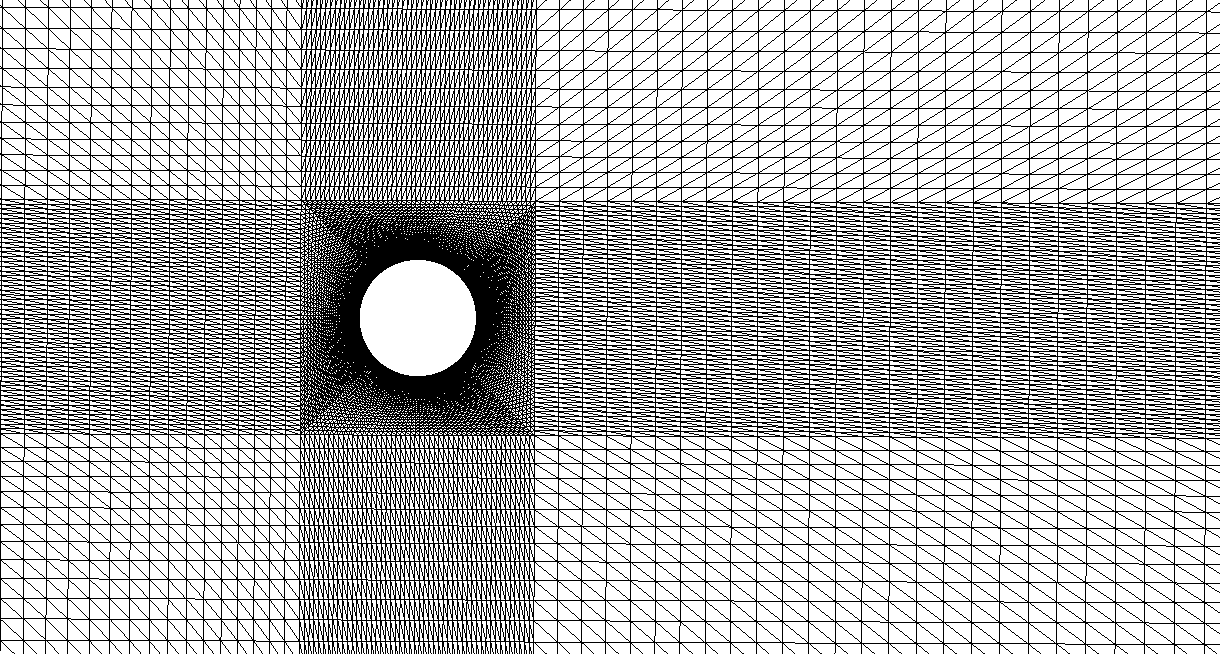
\includegraphics[width=.9\columnwidth]{mesh.png}
%   \end{center}
%   \caption{General and detailed views of the mesh used for the baseflow computation and subsequent analysis, the circular cylinder is submerged a depth $h$.}
% \end{figure}

%=====================================================================================
\section{Results}
\label{S:Results}
%=====================================================================================

In our case the liquid (bottom fluid) density and fluid viscosity is 100 times their respective top fluid value.

The first thing to do is to search a steady state solution of the Navier-Stokes equations, for the space of parameters of the problem $Re,Fr,h/D$. In this letter we have analyzed a range of Reynolds numbers close to the first Hopf bifurcation that appears in the absence of free surface. This range is $Re=(30,70)$ while the Froude number has been kept fixed to $Fr=3$ and the water depth was $h=?$. The horizontal and vertical velocity components of the baseflow and the free surface position corresponding to the case $Re=45$ and $Fr=3$ are shown in figures \ref{f:baseflow} and \ref{f:VOF}. The free surface elevation at the top of the cylinder is similar to the one presented by Bouscasse in \cite{Bouscasse14} but of course the wake is different due to the Reynolds number difference.

\begin{figure}[ht]
  \centering
    \subfloat[x-velocity from -0.15 (blue) to 2.15 (red)]{
	  \label{uRe45}
	  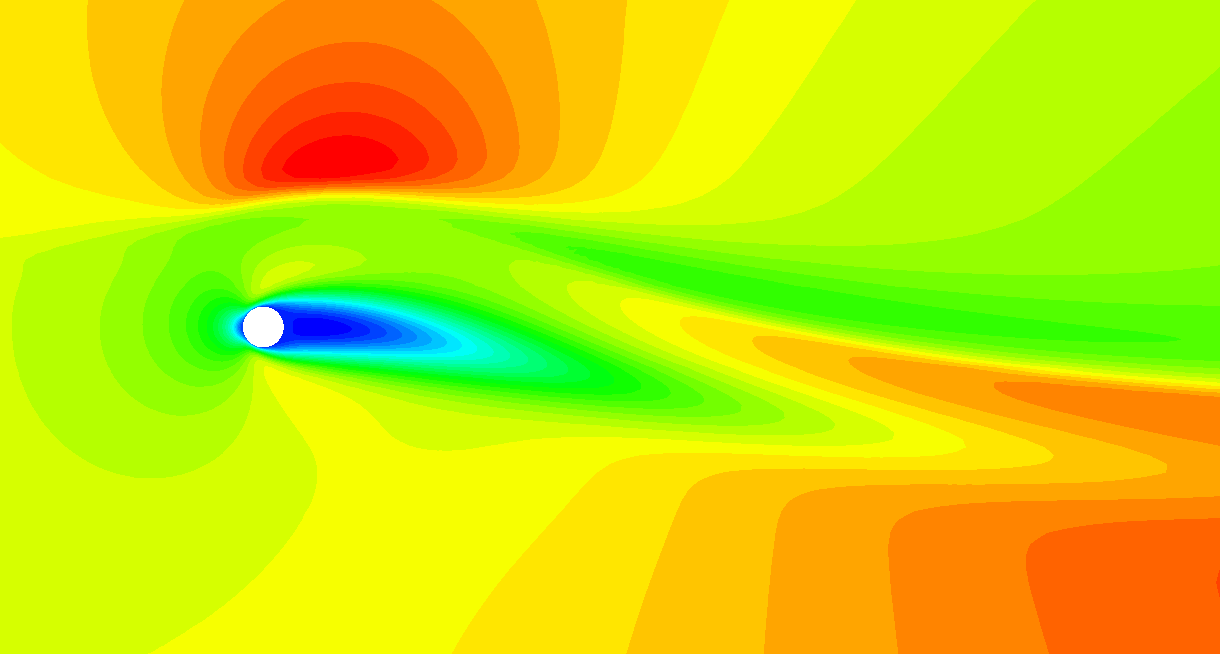
\includegraphics[width=.9\columnwidth]{uRe45.png}
    } \\
    %%----segunda subfigura----
    \subfloat[y-velocity from -0.65 (blue) to 0.75 (red)]{
	  \label{vRe45}
	  %\includegraphics[width=.9\columnwidth]{mesh_new.eps}
	  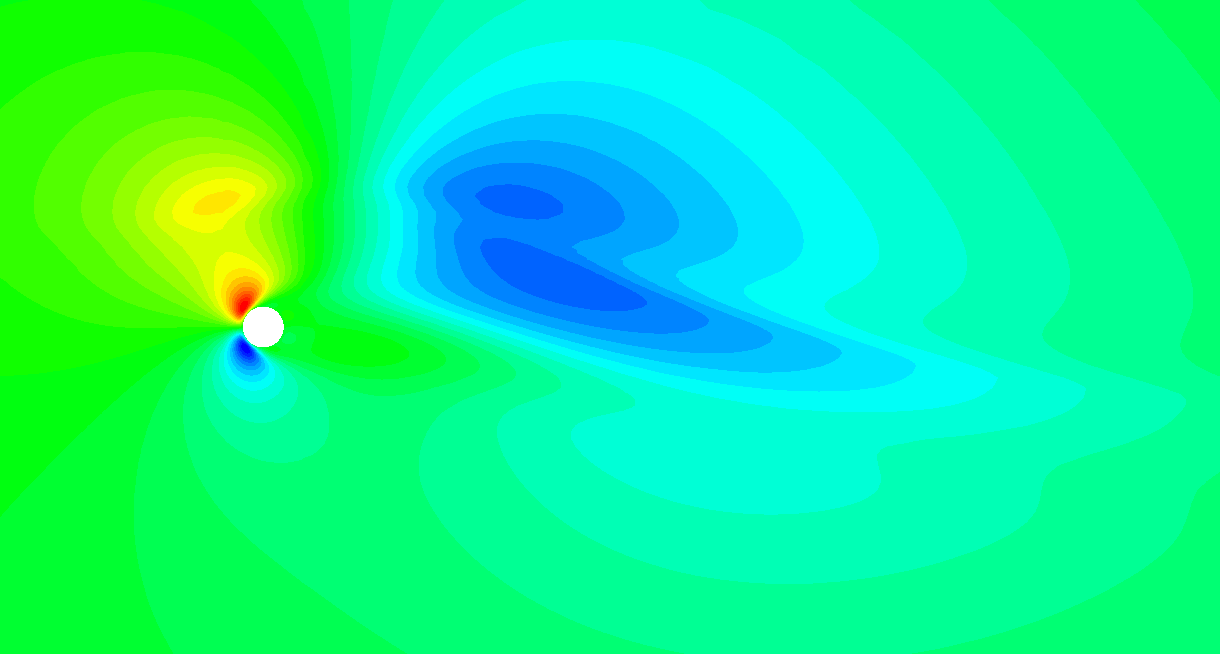
\includegraphics[width=.9\columnwidth]{vRe45.png}
    }
   \caption{Velocity representation at the steady state for $Re=45$ and $Fr=3$}
   \label{f:baseflow}
\end{figure}

 \begin{figure}
  \begin{center}
  %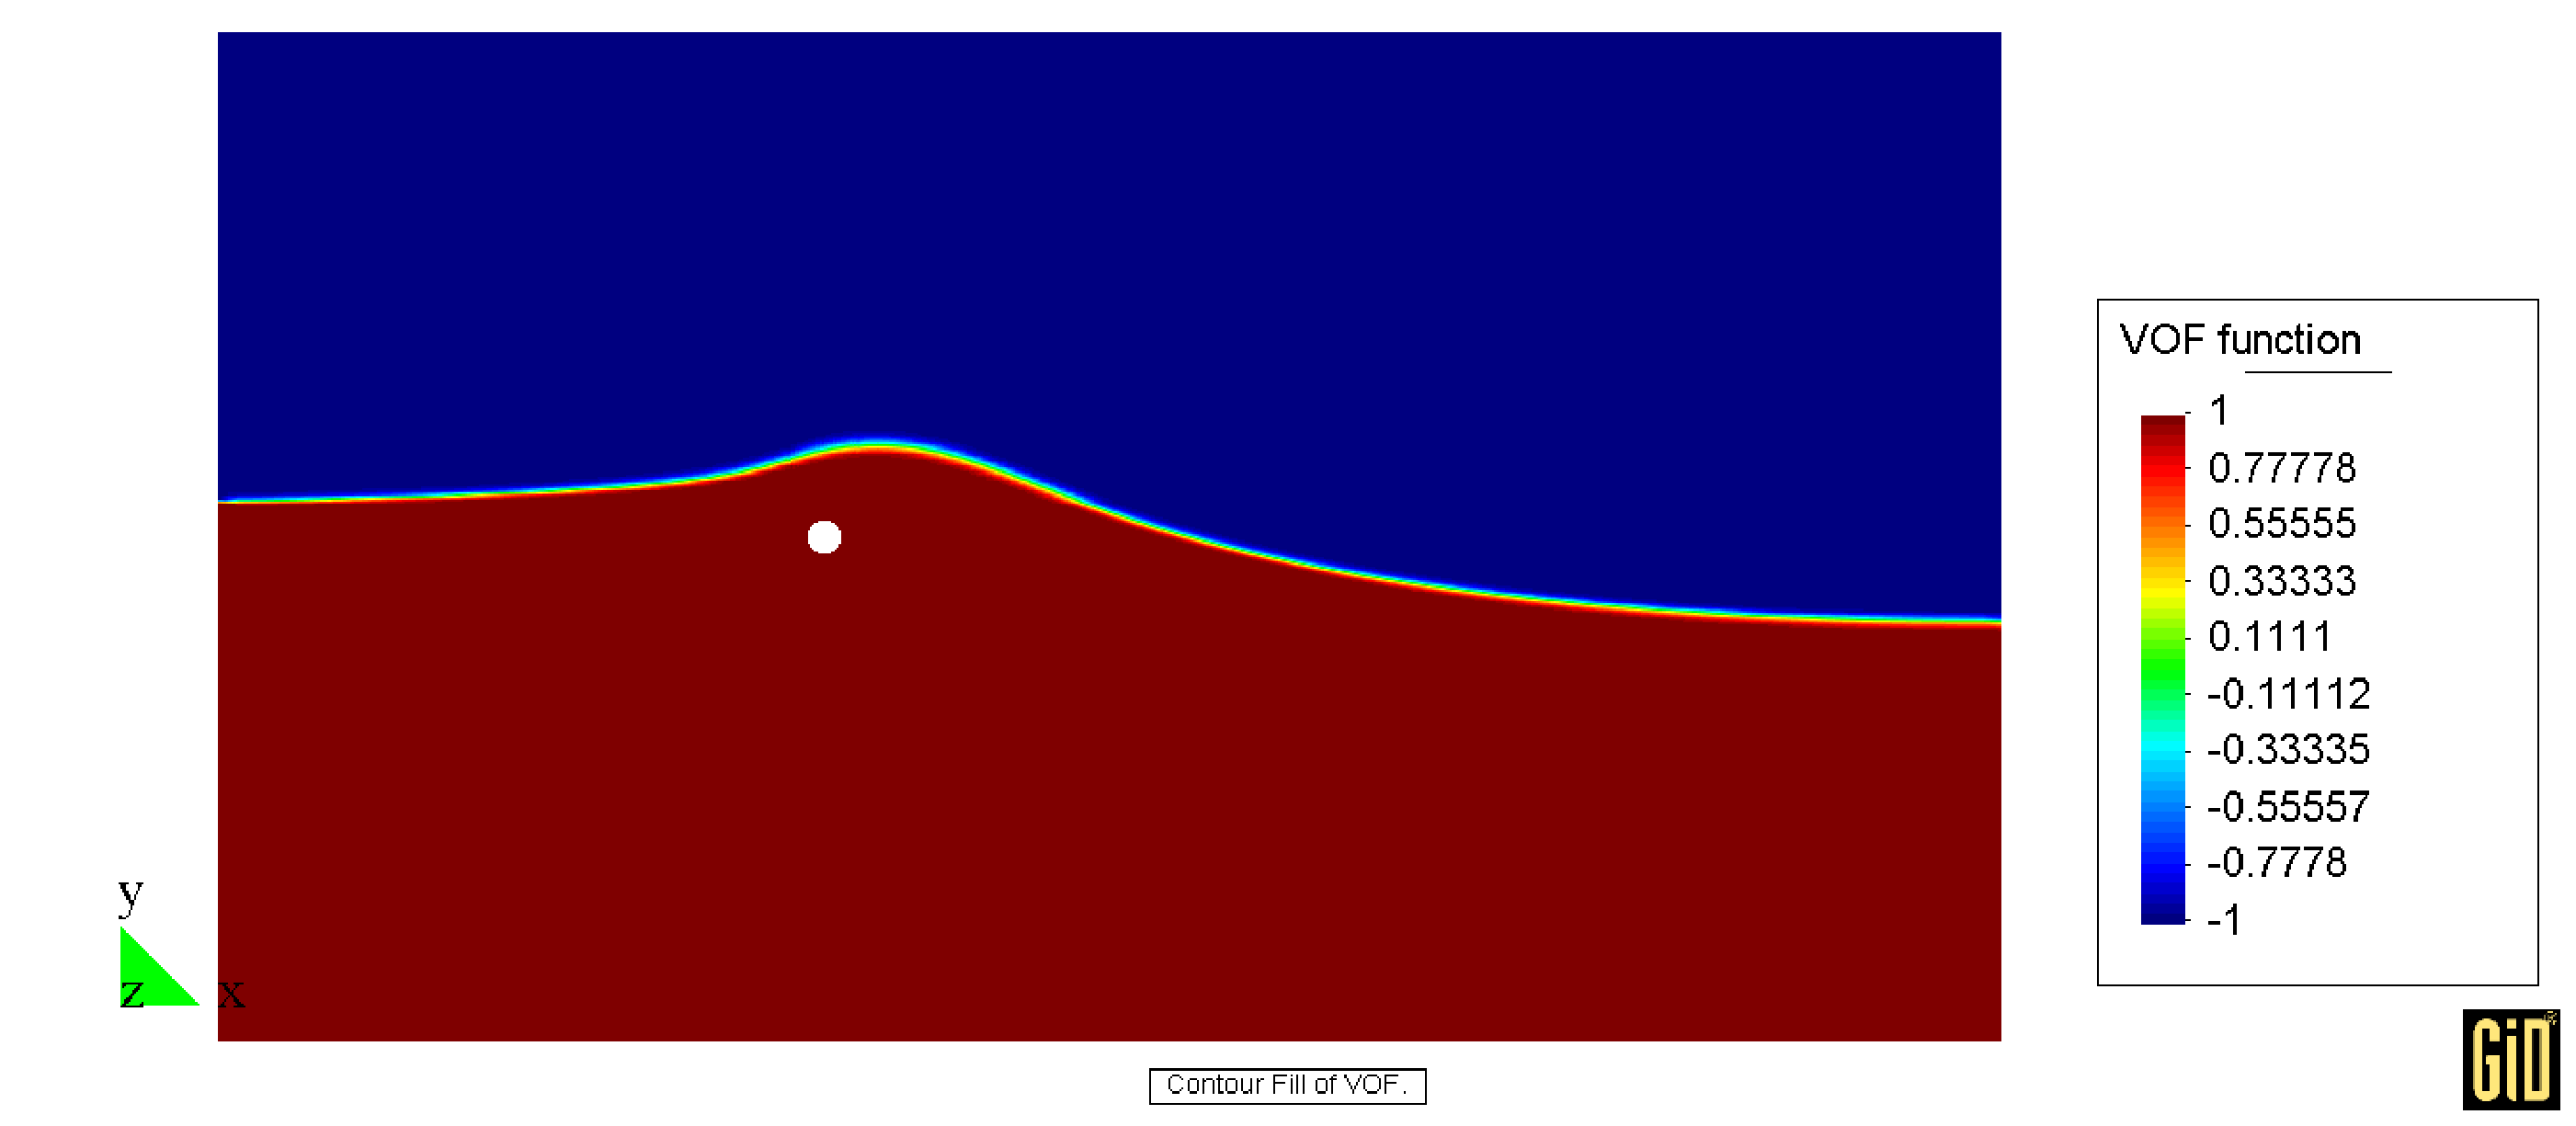
\includegraphics[width=6cm]{VOF.eps}\\
  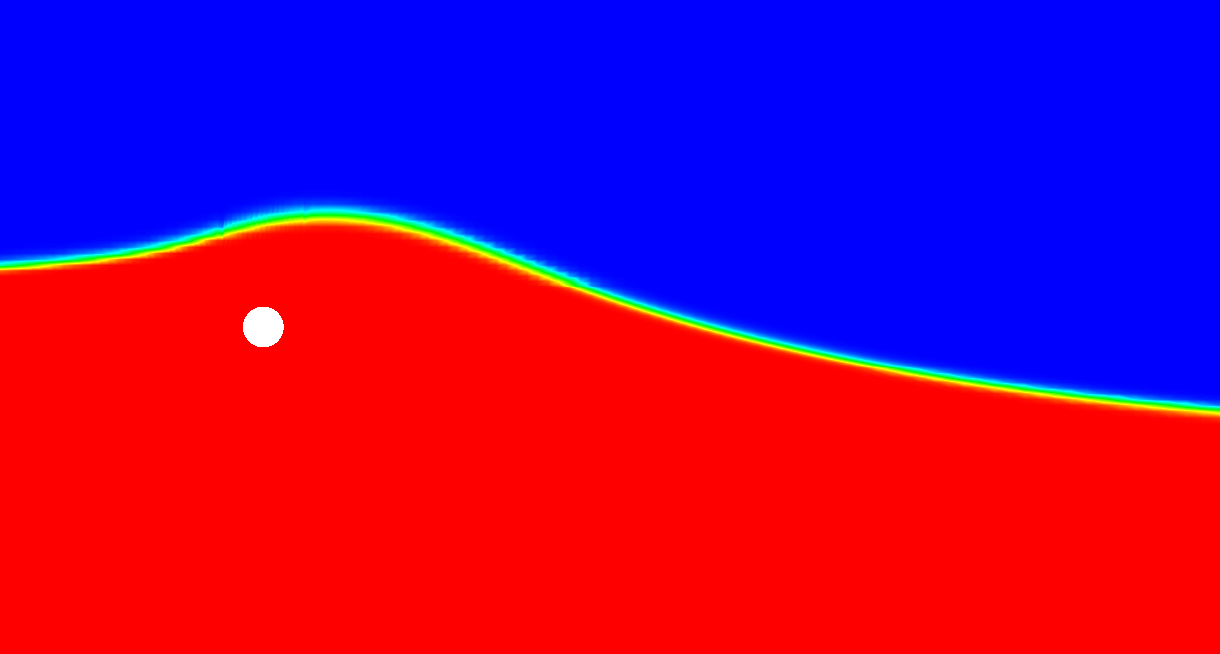
\includegraphics[width=.9\columnwidth]{vofRe45.png}
  \end{center}
  \caption{Free surface representation of the VOF scalar function at the steady state for $Re=45$ and $Fr=3$}
  \label{f:VOF}
\end{figure}

\begin{figure}
  \begin{center}
  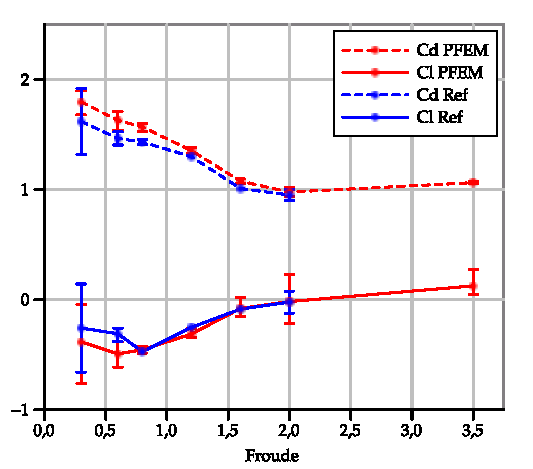
\includegraphics[width=6cm]{CdCl_Re180_hd_0_55.pdf}\\
  \end{center}
  \caption{Drag and Lift coefficients calculated with PFEM-2 compared with the reference work of Bouscasse \cite{Bouscasse14}. $Re=180$.} \label{f:CdCl}
\end{figure}



A collection of steady baseflows has been obtained varying the Reynolds number for $Re=30,40,45,50,60,70$. For the sake of code validation, the global drag and lift forces have been compared against previous results\cite{Bouscasse14} at the standard $Re=180$ and different Froude numbers being the agreement very satisfactory, see figure \ref{f:CdCl}. For each one a stability analysis based of the resolution of the large eigenvalue problem mentioned before has been done, and the evolution of the most unstable mode has been monitored. The evolution of the growth/damping rate and the angular frequencies of the most unstable mode for these Reynolds numbers is shown in figure \ref{f:omegas}. It can be observed that similarly to what happens in the absence of free surface the most unstable mode moves towards the unstable region $\omega_r<0$ when the Reynolds number is increased. For a Reynolds number very close to the one found in the absence of free surface $Re_c\approx 47$ the mode turns to be unstable a the vortex shedding appears in the flow. This frequency can be confirmed when the global force is monitored while the Navier-Stokes equations are solved, see figure \ref{f:lifts}. An increasing oscillation is appreciated once the critical Reynolds number $Re_c$ is exceeded. The novelty comes from the fact that the frequency associated to this oscillating unstable mode $\omega_= 0.98$ is higher when compared to the case without free surface aprox. 0.7, this frequency shift implies that the mode oscillation is clearly accelerated by the presence of the free surface.


\begin{figure}
  \begin{center}
    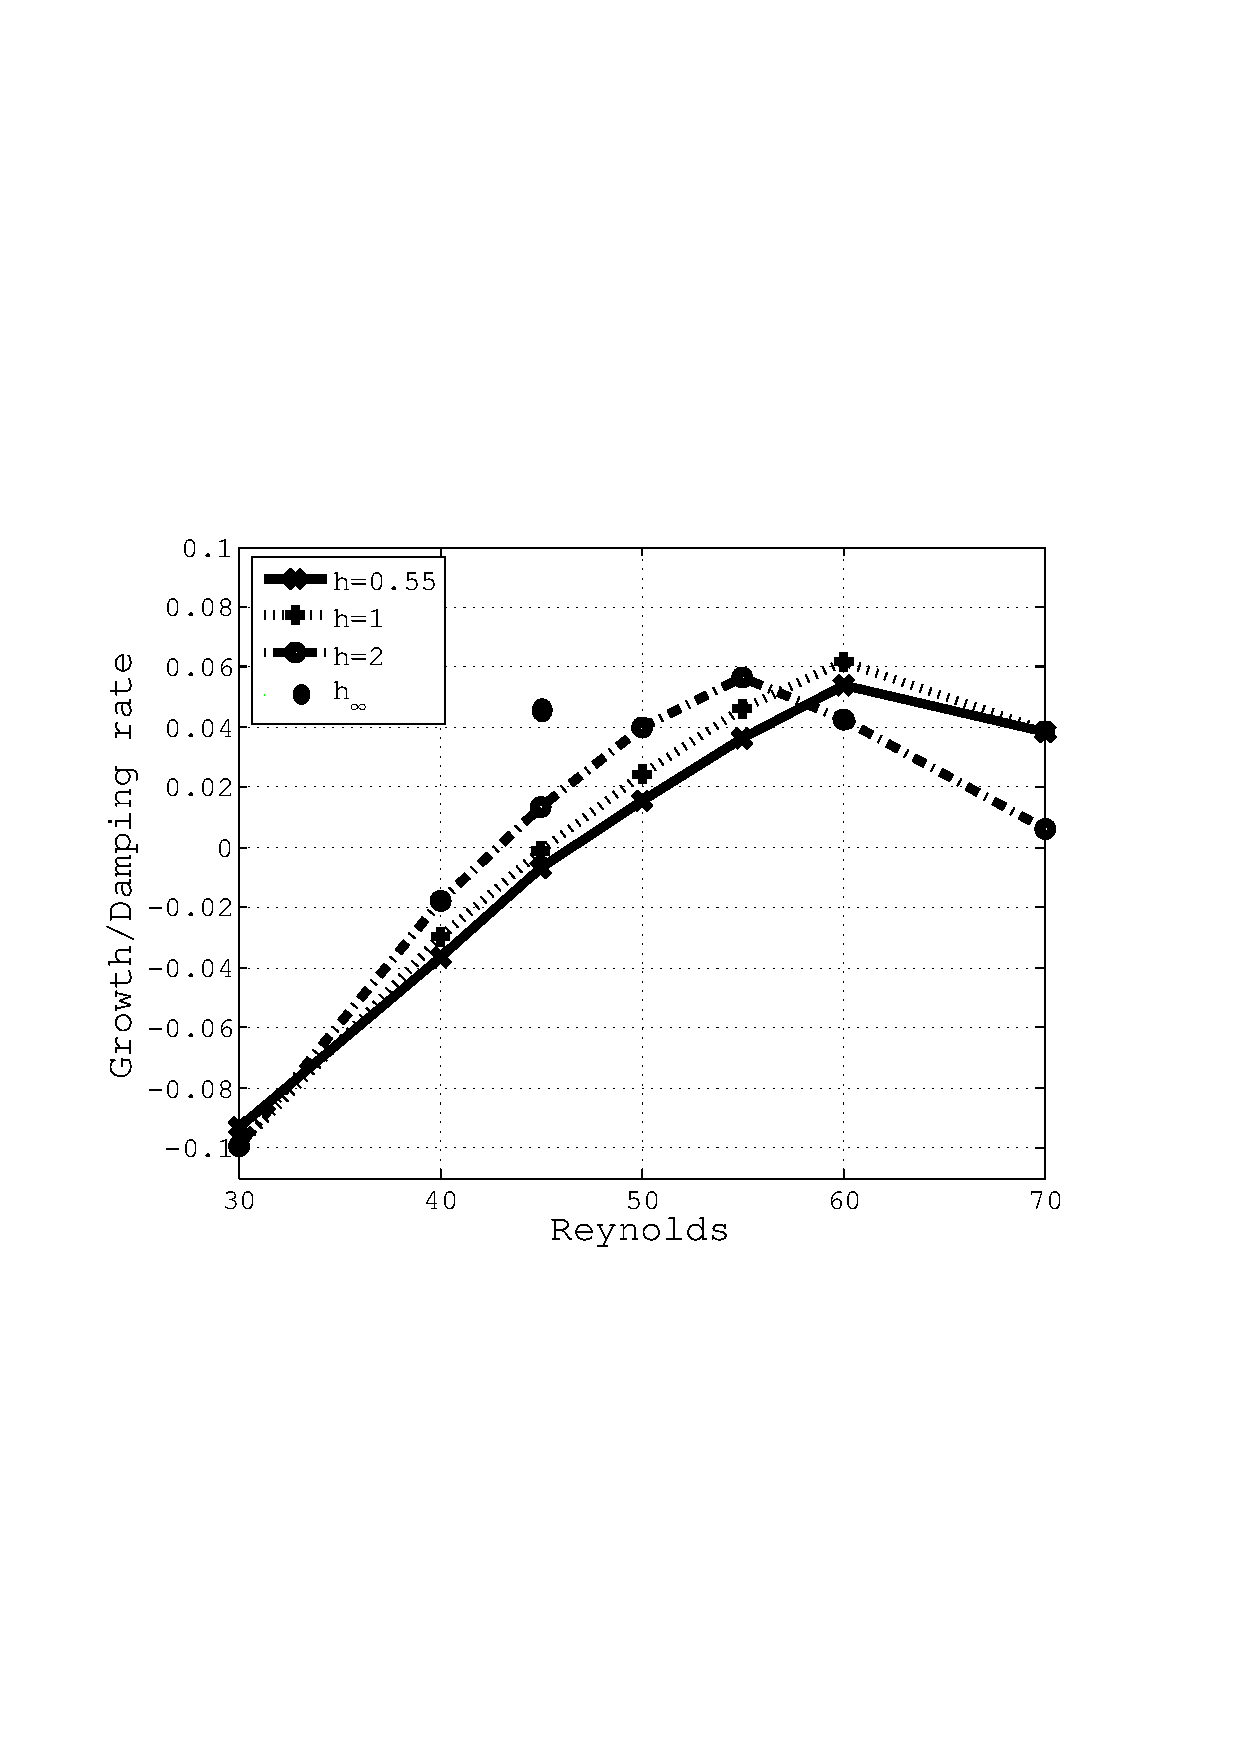
\includegraphics[width=5cm]{Growth.pdf}
    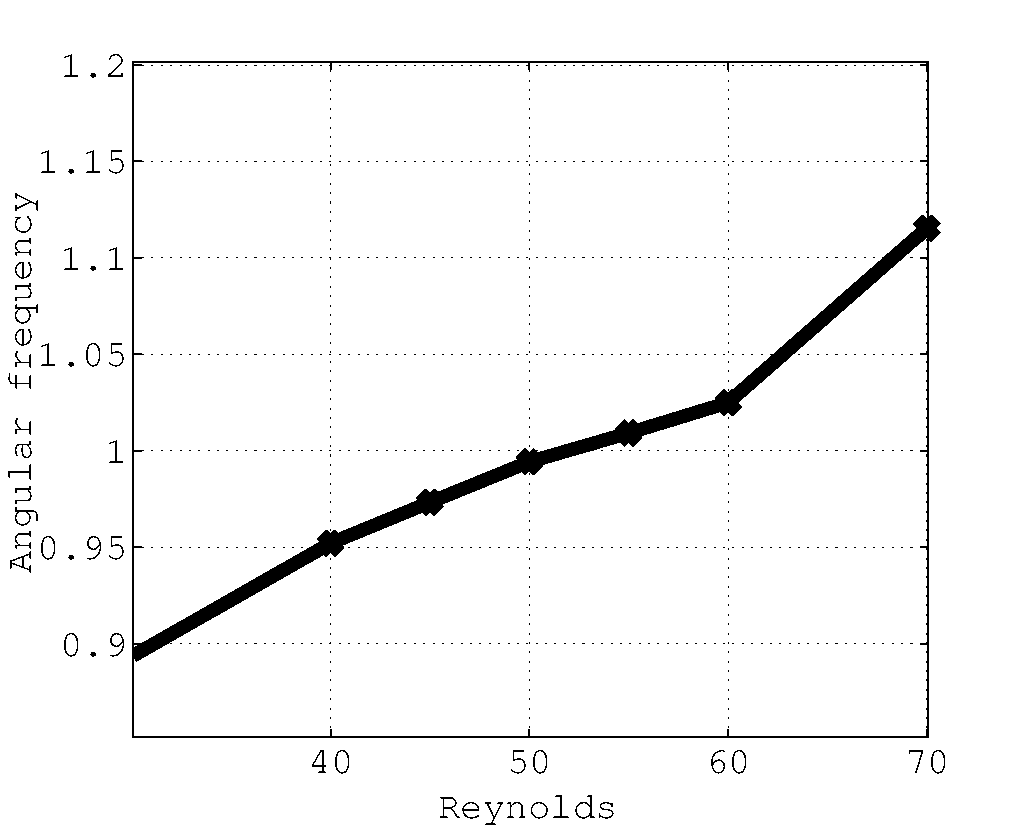
\includegraphics[width=5cm]{Freq.pdf}\\
  \end{center}
  \caption{Growth rate $Fr=3$}
  \label{f:omegas}
\end{figure}

\begin{figure}
  \begin{center}
  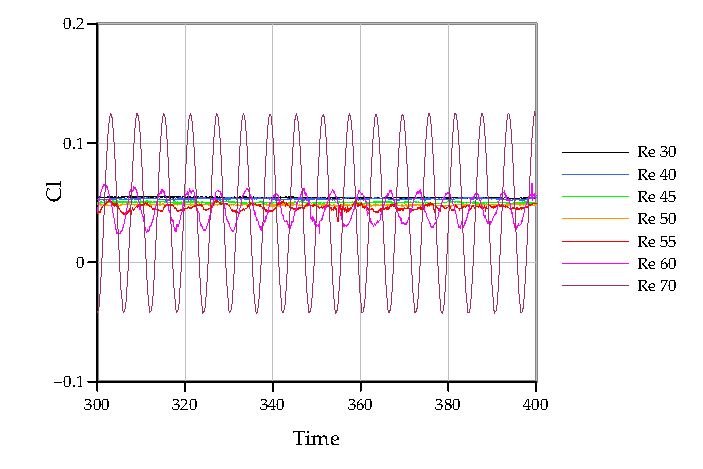
\includegraphics[width=\columnwidth]{Cl_Fr3_0.pdf}
  \end{center}
  \caption{Lift force at different Reynolds numbers.}
  \label{f:lifts}
\end{figure}

The mode corresponding to this oscillating unstable mode is shown in figure \ref{f:mode}, where the shape of the mode follows the tendency described by the free surface position.

\begin{figure}[ht]
  \centering
    \subfloat[x-velocity from -0.1 (blue) to 0.1 (red)]{
	  \label{pertuRe45}
	  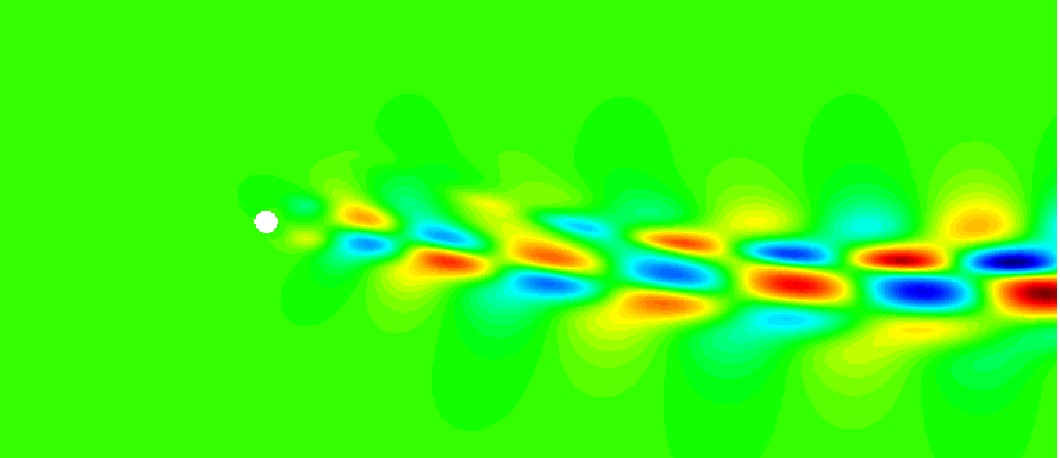
\includegraphics[width=.9\columnwidth]{pertuRe45.png}
    } \\
    %%----segunda subfigura----
    \subfloat[y-velocity from -0.008 (blue) to 0.007 (red)]{
	  \label{pertvRe45}
	  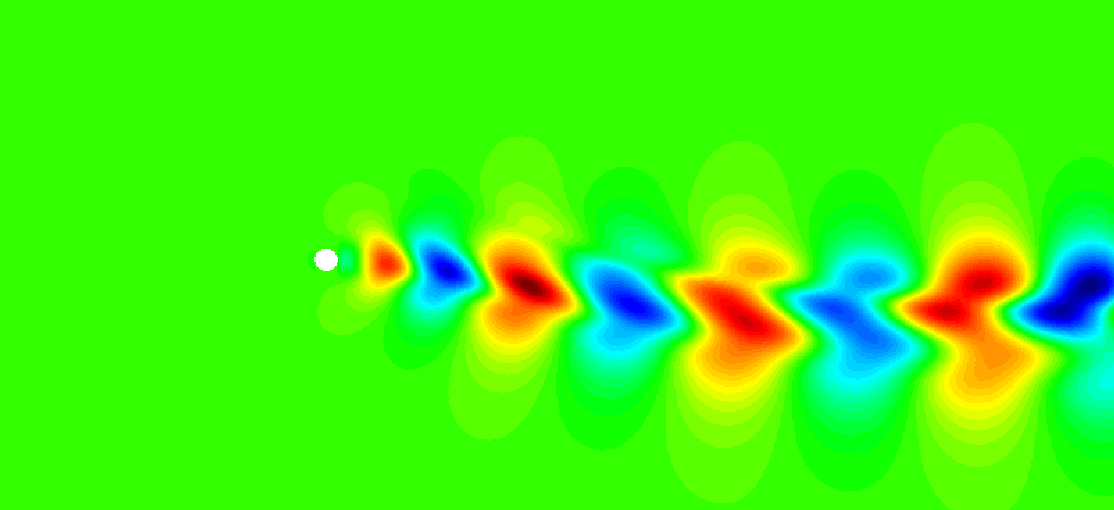
\includegraphics[width=.9\columnwidth]{pertvRe45.png}
    }
  \caption{Unstable mode $Re=45$ $Fr=3$}
  \label{f:mode}
\end{figure}

% \begin{figure}
%   \begin{center}
%   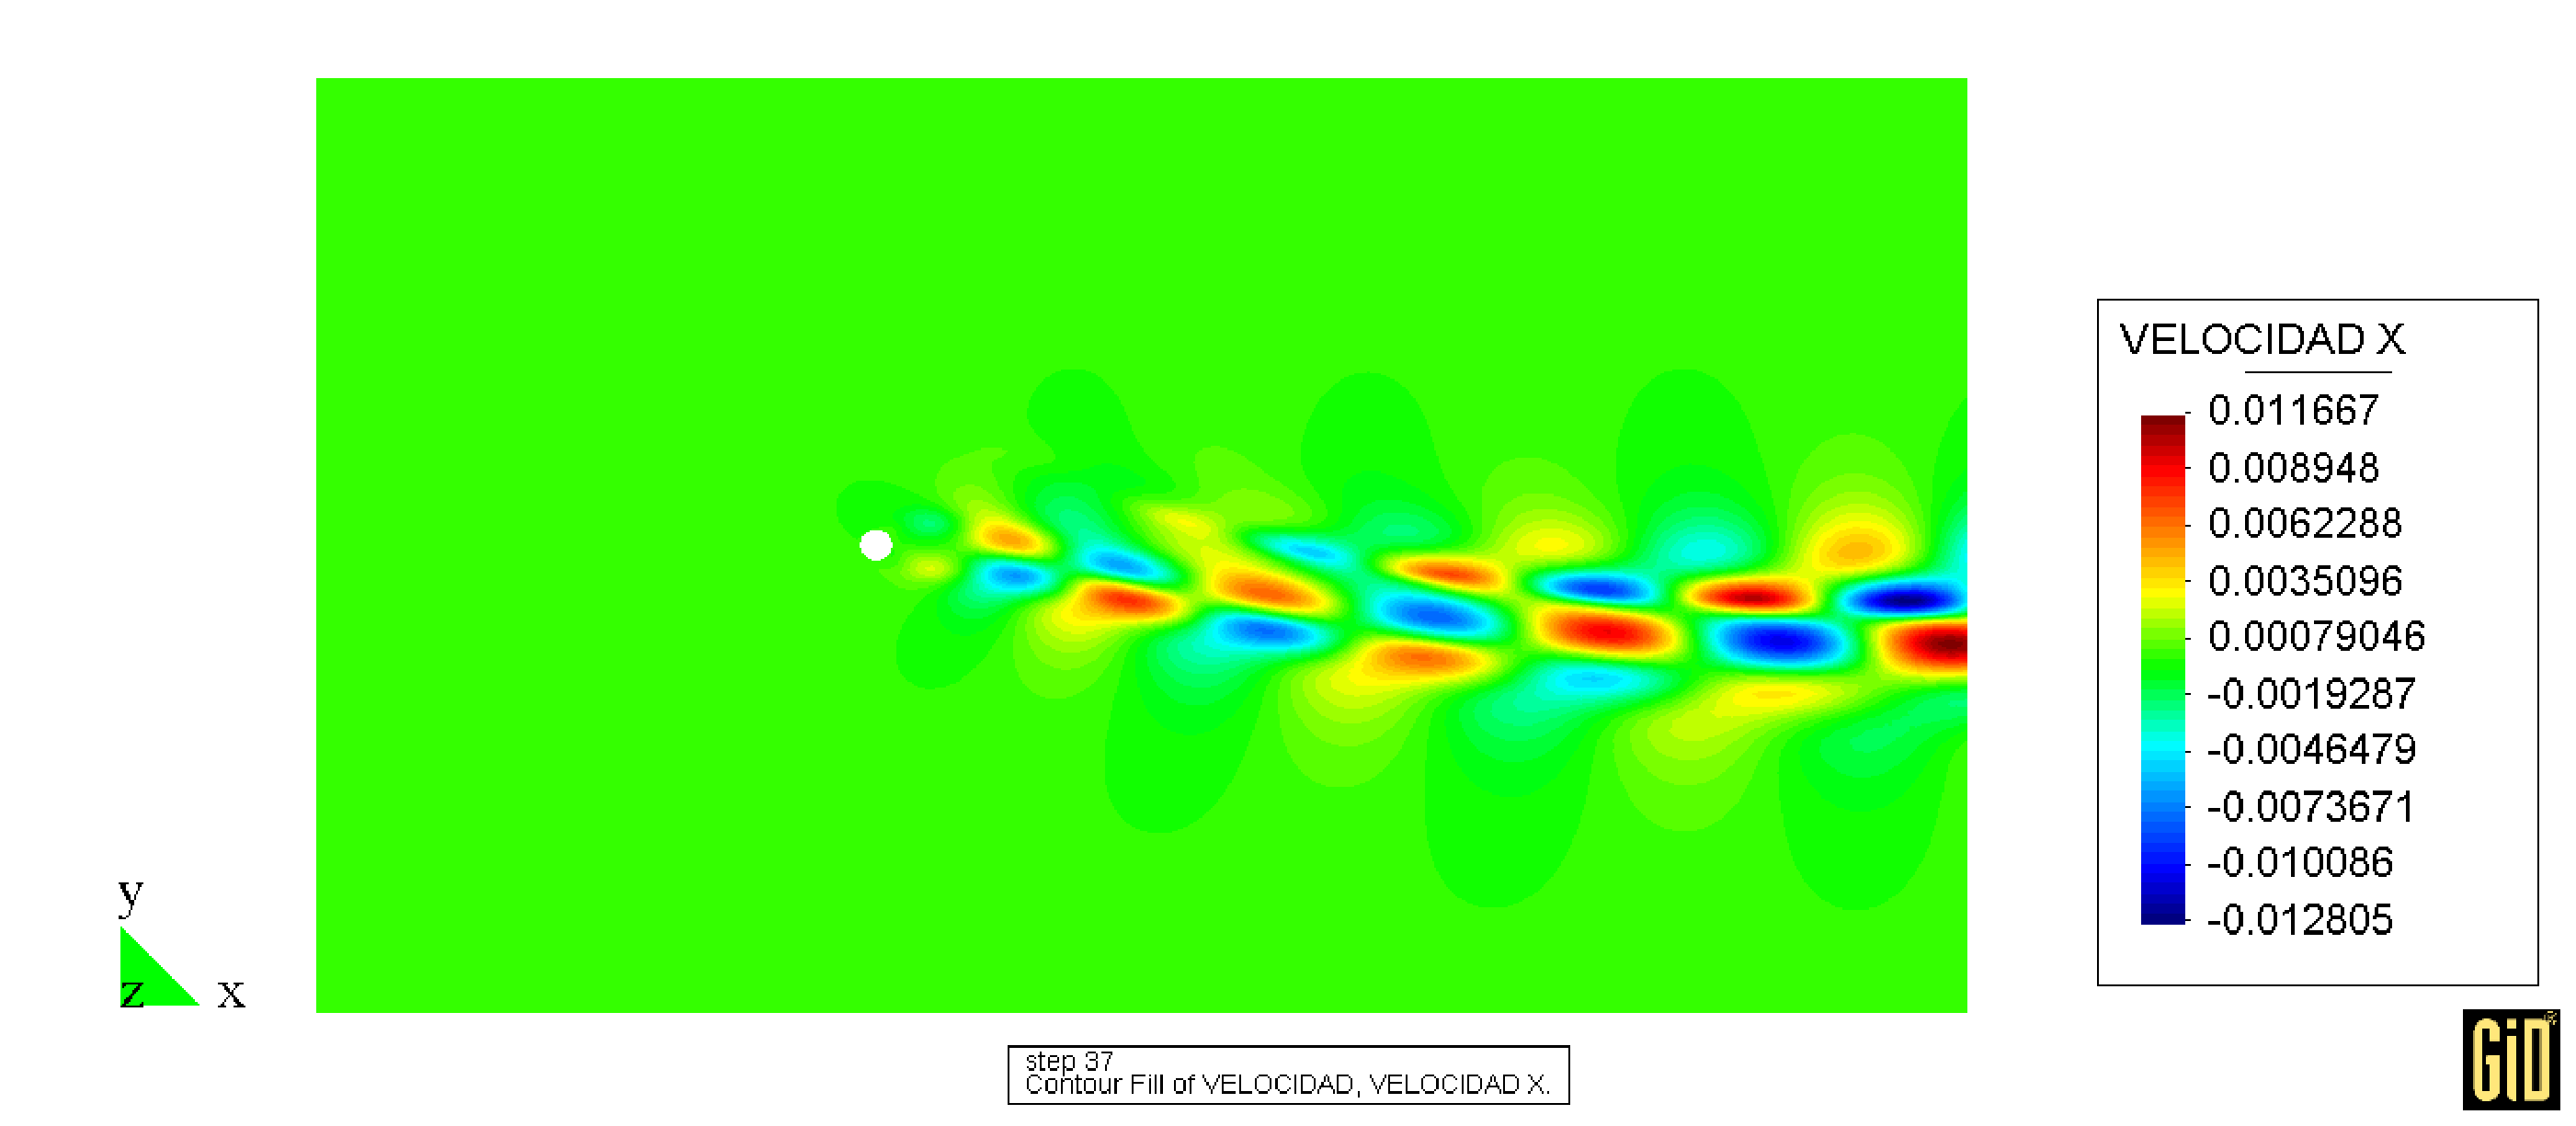
\includegraphics[width=6cm]{pertuRe45.eps}
%   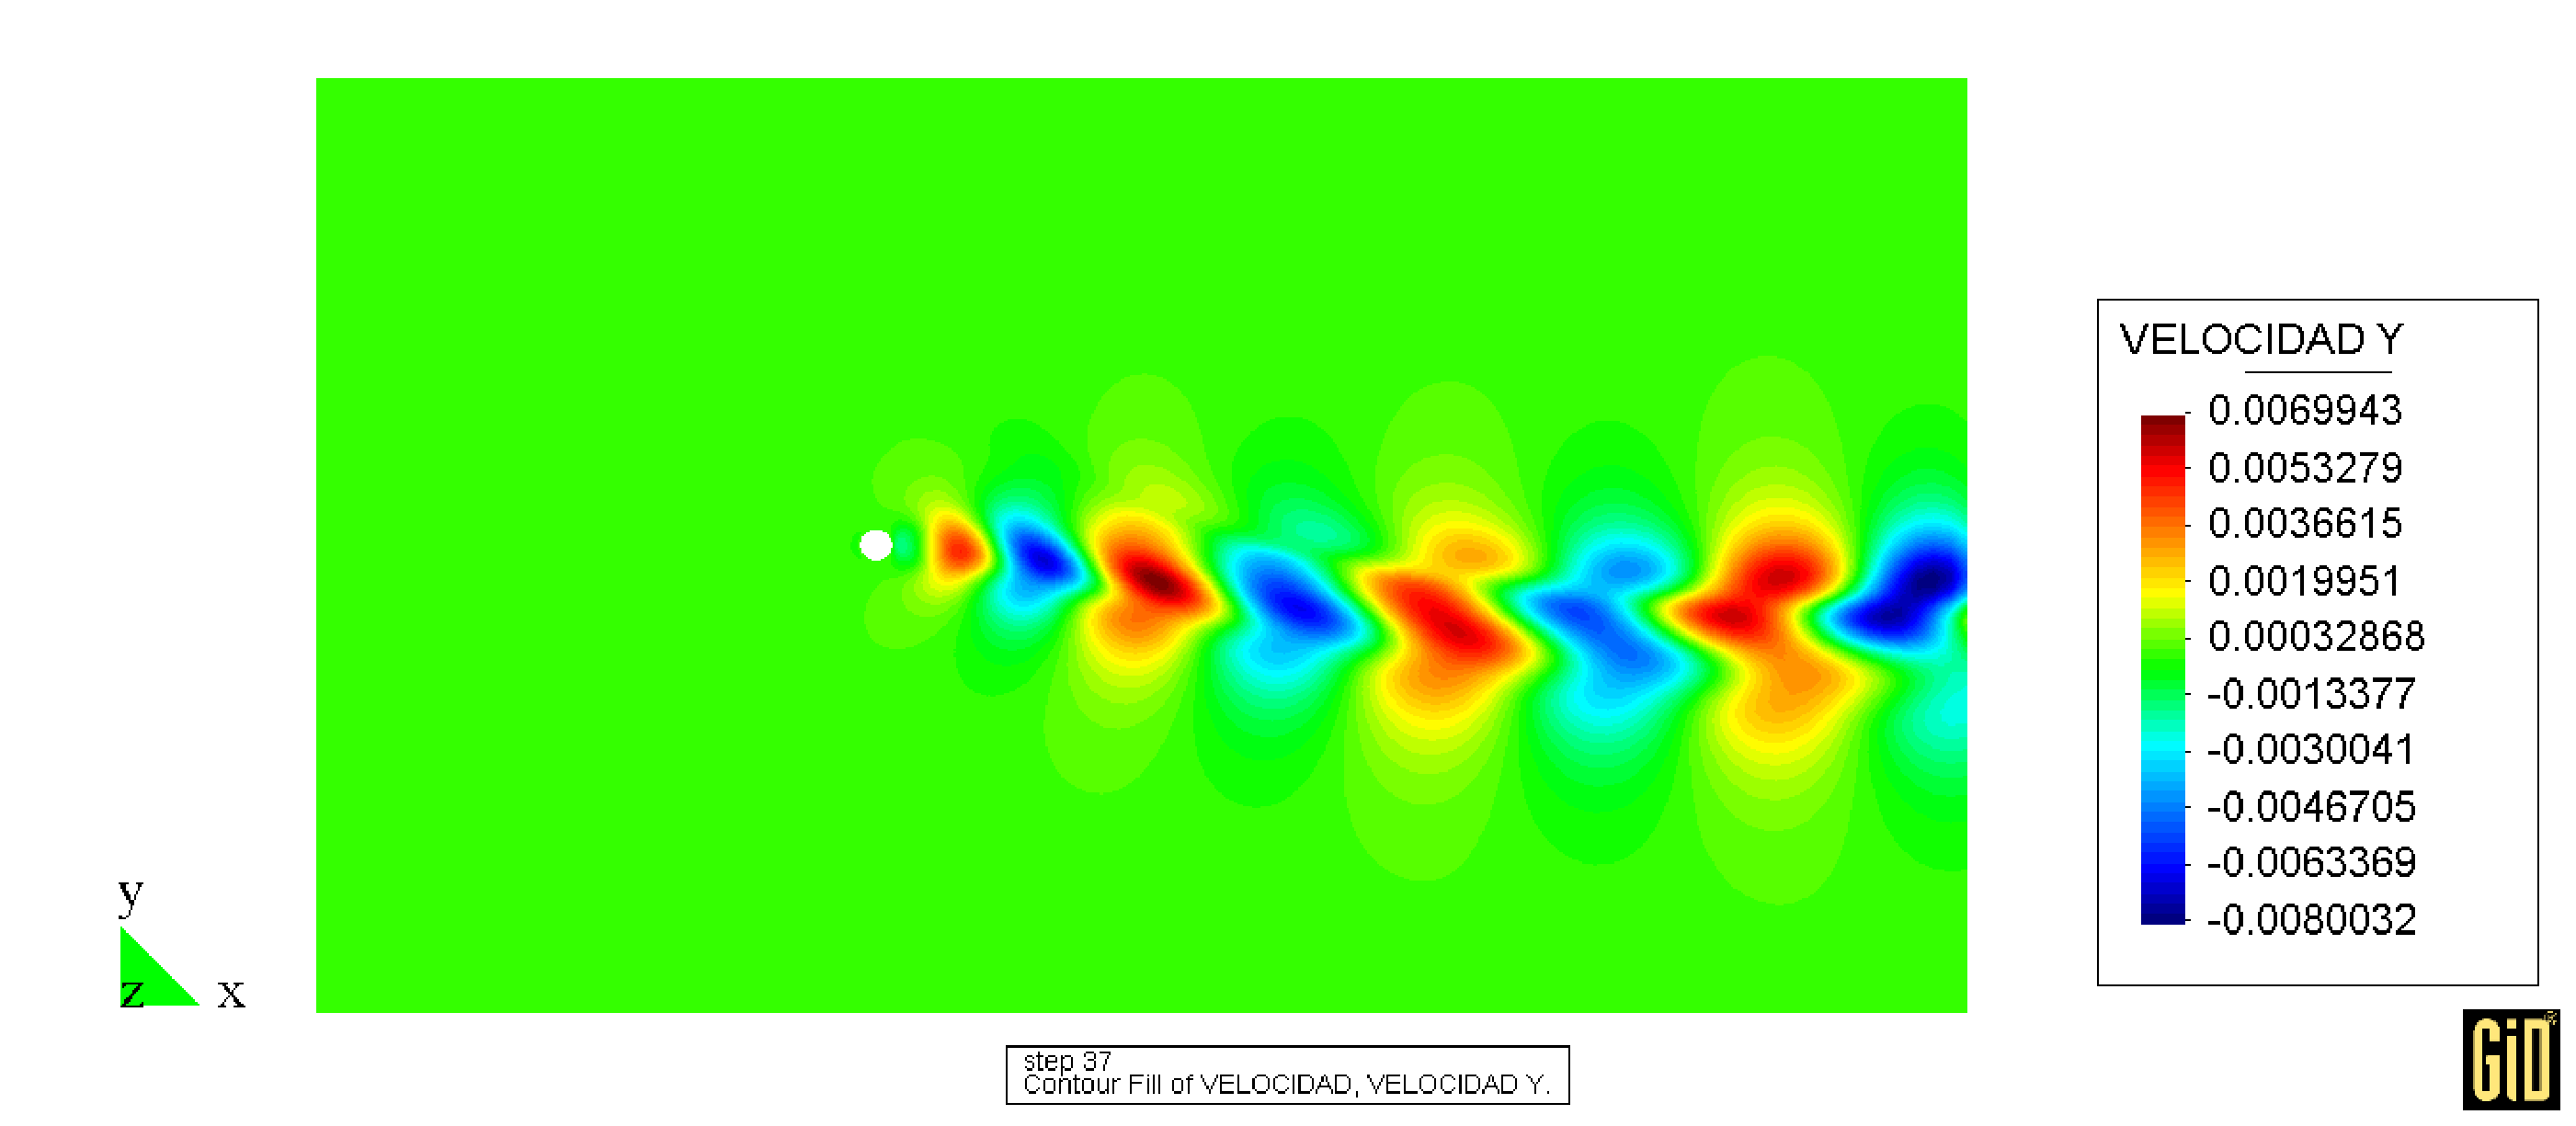
\includegraphics[width=6cm]{pertvRe45.eps}\\
%   \end{center}
%   \caption{Unstable mode $Re=45$ $Fr=3$}
%   \label{f:mode}
% \end{figure}

According to Dimas results when the Froude number is above 2.5 as in our case the Branch II becomes dominant and instability becomes of the absolute type.\cite{Dimas89}


In the future these results will be also confirmed and extended to higher Reynolds values by a Dynamic Mode Decomposition. Also the possibility of having situations such that growing instabilities caused by the free surface oscillations could also included in the analysis, similar to what occurs in a Rayleigh-Taylor instability. The possibility will be studied in future works.
It is believed that the theoretical findings of this Letter can be realized by experiments and confirmed by 3D simulations. This work was supported by the Technical University of Madrid by the project (PID) "Combination of Eulerian and Lagrangian methodologies for the solution of free surface flows."


\bibliography{mybib}

\end{document}

% body of paper here - Use proper section commands
% References should be done using the \cite, \ref, and \label commands
\section{}
% Put \label in argument of \section for cross-referencing
%\section{\label{}}
\subsection{}
\subsubsection{}

% If in two-column mode, this environment will change to single-column
% format so that long equations can be displayed. Use
% sparingly.
%\begin{widetext}
% put long equation here
%\end{widetext}

% figures should be put into the text as floats.
% Use the graphics or graphicx packages (distributed with LaTeX2e)
% and the \includegraphics macro defined in those packages.
% See the LaTeX Graphics Companion by Michel Goosens, Sebastian Rahtz,
% and Frank Mittelbach for instance.
%
% Here is an example of the general form of a figure:
% Fill in the caption in the braces of the \caption{} command. Put the label
% that you will use with \ref{} command in the braces of the \label{} command.
% Use the figure* environment if the figure should span across the
% entire page. There is no need to do explicit centering.

% \begin{figure}
% \includegraphics{}%
% \caption{\label{}}
% \end{figure}

% Surround figure environment with turnpage environment for landscape
% figure
% \begin{turnpage}
% \begin{figure}
% \includegraphics{}%
% \caption{\label{}}
% \end{figure}
% \end{turnpage}

% tables should appear as floats within the text
%
% Here is an example of the general form of a table:
% Fill in the caption in the braces of the \caption{} command. Put the label
% that you will use with \ref{} command in the braces of the \label{} command.
% Insert the column specifiers (l, r, c, d, etc.) in the empty braces of the
% \begin{tabular}{} command.
% The ruledtabular enviroment adds doubled rules to table and sets a
% reasonable default table settings.
% Use the table* environment to get a full-width table in two-column
% Add \usepackage{longtable} and the longtable (or longtable*}
% environment for nicely formatted long tables. Or use the the [H]
% placement option to break a long table (with less control than
% in longtable).
% \begin{table}%[H] add [H] placement to break table across pages
% \caption{\label{}}
% \begin{ruledtabular}
% \begin{tabular}{}
% Lines of table here ending with \\
% \end{tabular}
% \end{ruledtabular}
% \end{table}

% Surround table environment with turnpage environment for landscape
% table
% \begin{turnpage}
% \begin{table}
% \caption{\label{}}
% \begin{ruledtabular}
% \begin{tabular}{}
% \end{tabular}
% \end{ruledtabular}
% \end{table}
% \end{turnpage}

% Specify following sections are appendices. Use \appendix* if there
% only one appendix.
%\appendix
%\section{}

% If you have acknowledgments, this puts in the proper section head.
%\begin{acknowledgments}
% put your acknowledgments here.
%\end{acknowledgments}

% Create the reference section using BibTeX:
\bibliography{basename of .bib file}

\end{document}
%
% ****** End of file apstemplate.tex ******

